 %%%%Textart%%%%
\documentclass[a4paper, 12pt, oneside]{scrbook}

%Alle packages, commands, etc ausgelagert in mystyle.sty
\usepackage{mystyle}



\begin{document}

\begin{titlepage}
\begin{center}
\vspace*{2cm}
{\huge Semantic Image Synthesis with Score-Based Generative Models} 
\vspace{2cm}\\
{\large by\\Tim Küchler}
\vspace{2cm}\\
{Professor Björn Ommer, Advisor}
\vfill
A thesis submitted in partial fulfillment\\
of the requirements for the\\
Degree of Bachelor of Arts with Honors\\
in Physics
\vspace*{3cm}
Ruprecht Karl University of Heidelberg\\
Heidelberg, Germany\\
\today % 
\end{center}
\end{titlepage}
%
\frontmatter 
\chapter{Abstract}
\begin{center}

\end{center}

\chapter{Acknowledgments}

\tableofcontents

\mainmatter
\chapter{Introduction}
\section{Generating realistic data} %0.5-1

\section{Semantic Segmentation and Semantic Synthesis} %0.5-1
\section{Score-Based Models - The new contenders to GANs?} %0.5-1

\chapter{State of the art}
\section{Semantic Segmentation} %0.5-1
\subsection{Introduction}
\subsection{U-Net} %1-2
\subsection{FCN}
\subsection{Dense}
\subsection{FC Dense} 
\section{Generative models - GANs, VAEs and Co.} %0.5-1
\subsection{Introduction}
\subsection{Generative Adversarial networks (GANs)} %4-6
\subsection{Variational Autoencoders (VAEs) (eher kurz in 2.2.4)} %1-1.5
\subsection{Other Generative Models} %0.5-1

\chapter{Score-Based Generative Models} %5-7
\chaptermark{SGM}

\section{Semantic Segmentation} \label{sec:3.1}
A large field of models in Deep Learning are discriminative models. A simple version of a discriminative model would be a classifier. A classifier given an input $\vec{x}$ outputs a scalar class value $y\in\vec{y}$ of the input where $\vec{y}$ is a set of classes (which are also called labels). The simplest classifier would be a binary classifier that places an input into one of two classes, e.g. deciding if an image shows a cat or a dog. More advanced classifiers identify way more classes. A classical example would be a classifier trained on the CIFAR-10 dataset \cite{cifar10}, which contains millions of $32\times32$ pixel images categorized by 10 classes (car, airplane, dog, $\dots$).

The above described classifiers always assign one scalar value to an input. Semantic Segmentation Networks also assign scalar values, but not one value per image, but one value per pixel! This already reveals a lot about the application of such networks. They operate on images and their task is to assign each pixel in the image a class. For example, given the image of a street scene a semantic segmentation network tries to classify each individual pixel as part of a car, a street, a building, $\dots$\,.

There are also modifications of semantic segmentation for example instance segmentation. In instance segmentation, not only is each pixel assigned a class, but also the different instances of objects in an image are specified. An overview of semantic segmentation and related techniques is shown in \hyperref[fig:3.1]{Fig.\,3.1}
%
\begin{figure} \label{fig:3.2}
    \centering
    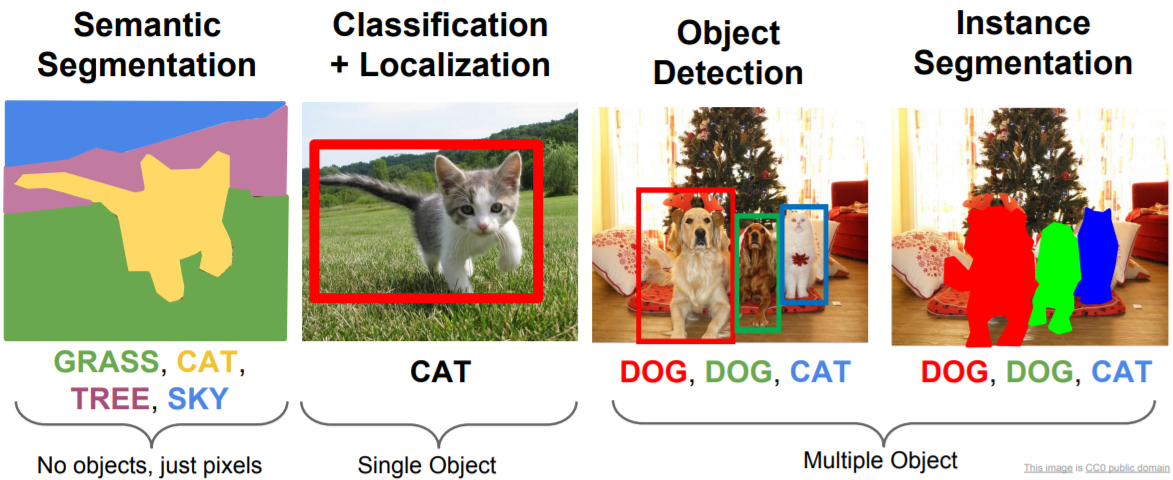
\includegraphics[width=.8\textwidth]{Chapters/figures/sem_seg.PNG}
    \caption{Overview of various computer vision tasks}
\end{figure}
%

As we will see in \hyperref[sec:4.5]{Sec.\,4.5} and \hyperref[chap:5]{Chapter 5}, semantic segmentation networks are necessary to make semantic image synthesis possible with Score-Based Generative Models. Therefore, those models used in later work are briefly explained below:

\subsection{FCN}
\subsection{U-Net} %1-2

%%%%%%%%%%%%%%%%%%%%%%%%%%%%%%%%%%%%%%%%%%%%%%%%%%%%%%%%%%%%%%%%%%%%%%%%%%%%%%%%%%%%%%%%%%%%
\section[Generative Modeling – VAEs and GANs]{Generative Modeling – VAEs and GANs%
    \sectionmark{Generative Modeling}}
\sectionmark{Generative Modeling}
There are mainly two types of models: \textit{Generative Models} and \textit{Discriminative Models}. The latter discriminate between different kind of data instances, e.g. discriminate images of cats and dogs. Semantic Segmentation Models (\hyperref[sec:3.1]{Sec.\,3.1}) are discriminative models. Given a data instance $\vec{x}$ and a set of labels $\vec{y}$ conditional models learn the conditional probability $p(\vec{y}|\vec{x})$. Generative model generate new data instances. They capture the joint probability $p(\vec{x},\vec{y})$ or $p(\vec{x})$ if there are no labels. In general generative models are a lot harder than discriminate models. There are various approaches to generative modeling, the most popular being Variational Autoencoders (VAEs) and Generative Adversarial Networks (GANs).

\subsubsection{Variational Autoencoders}
Although VAEs \cite{vae_original} do not play a major role in this thesis, they are briefly discussed due to their strong influence in modern generative modeling. In order to understand VAEs one must first understand what an autoencoder is. Autoencoders tackle the problem of encoding and decoding data with minimum information loss. Data generally is classified by some abstract features which often form a high dimensional space. The task of an autoencoder is to learn to reduce the dimensionality of this high dimensional features by selecting important old features (selection) or creating less, new features based on the old features (extraction). The arising feature space is called \textit{latent space} which essentially only contains the most important features of the input data. To learn such an encoding the autoencoder network consists of an encoder network $E(\vec{x})$ and a decoder network $D(\vec{x})$. An input $\vec{x}$ is first encoded by the encoder to a low dimensional value $\vec{z}$ which then is decoded by the decoder to an output $\tilde{\vec{x}}$ of the same dimension as the input. Thereafter the input $\vec{x}$ is compared to the output $\tilde{\vec{x}}$ and the network gets punished for differences between input and output.

An autoencoder thus learns to compress and decompress data in the best possible way without loss of information. A na\"{i}ve way to now generate new data via a trained autoencoder is to use the decoder to decode a random sample from the latent space. The problem with this approach is that the autoencoder learns to best possible compress the data. As a consequence we cannot sample from the latent space because the distribution in latent space has no meaning w.r.t the real data. For example, if you decode the image of a car into the latent space and then change the latent representation of the car just a little, after decoding you will most likely see noise instead of an image of a new car. In mathematical terms the latent space of an autoencoder is not regularized.

A VAE solves this problem by ensuring that the latent space has good properties that enable generative modeling while still learning to encode the data in an efficient way. In order to do so the encoder of a VAE does not encode an input $\vec{x}$ to a single value but to a distribution in latent space $p(\vec{z}|\vec{x})$. The decoder then decodes a sample $\vec{z}\sim p(\vec{z}|\vec{x})$ to an output $\tilde{\vec{x}}$ which is compared to the output to compute a reconstruction loss. Furthermore a regularization loss is computed assuring that $p(\vec{z}|\vec{x})\sim\mathcal{N}(\vec{0},\vec{I})$. The regularized latent space has the very useful property that similar data is close together. So now if the decoder is given a slightly different latent representation of a car, it would decode it into a new image of a car. An overview of the VAE network architecture can be seen in \hyperref[fig:3.1]{Fig.\,3.1}
%
\begin{figure} \label{fig:3.2}
    \centering
    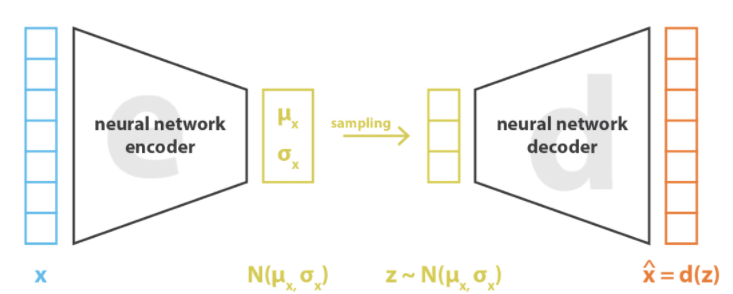
\includegraphics[width=.65\textwidth]{Chapters/figures/vae.PNG}
    \caption{Basic VAE model architecture}
\end{figure}
%
\subsubsection{Generative Adversarial Networks}
GANs were proposed in 2014 \cite{gan_original} and have since seen great success and a lot of adaptions. GANs work by combining two models: A generator model and a discriminator model. These two models are trained at the same time and have an adversarial relationship. Adversarial in that sense means that the generator and discriminator have opposing objectives. 

The generator $G(\vec{x})$ has the task of generating samples of the data distribution $p_{data}(\vec{x})$. The discriminator $D(\vec{x})$ has the role of distinguishing the generated data $\tilde{\vec{x}}$ from the real data $\vec{x}$. So to say the task of the generator is to best possible trick the discriminator that at the same time has the task to best possible decide if an image is real or fake (generated). If the discriminator correctly identifies a generated image as fake the generator is punished to produce better images. Obviously, "better" just means that the images are more likely to fool the discriminator, which does not necessarily equate to a real-looking image. When the discriminator is deceived by the generator, it is punished to better discriminate real and fake images. While the GANs can produce excellent samples and are fast at sampling, it's easy to imagine how hard it is to train two networks at the same time. If not properly adjusted training quickly becomes unstable.

The absolute error of the discriminator can be written in the following way:
%
\begin{equation}
    E(G,D)=\frac{1}{2}\left(\mathbb{E}_{\vec{x}\sim p_{t}}[1-D(\vec{x})]+\mathbb{E}_{\vec{x}\sim p_{z}}[D(G(\vec{z}))]\right)
\end{equation}
%
Here $\vec{x}$ is a input to the discriminator and $\vec{z}$ is a random input to the generator. Rewriting $G(\vec{z})$ as an input to the discriminator yields
%
\begin{equation} \label{equ:3.2}
    E(G,D)=\frac{1}{2}\left(\mathbb{E}_{\vec{x}\sim p_{t}}[1-D(\vec{x})]+\mathbb{E}_{\vec{x}\sim p_{g}}[D(\vec{x})]\right),
\end{equation}
%
where $\vec{x}$ can either be a real input ($\vec{x}\sim p_t$) or a generated input ($\vec{x}\sim p_g$). Therefore in \hyperref[equ:3.2]{Equ.\,3.2} the left term describes the error of falsely classifying a real image as generated and the right term describes the error of falsely classifying a generated image as real. From this it can be deduced that the perfect discriminator $D^*(\vec{x})$ classifies a real image as $1$ and a fake image as $0$. 

The total model objective of GANs can be written as 
%
\begin{equation}
    \underset{G}{\max}\left(\underset{D}{\min}\,E(G,D)\right),
\end{equation}
%
which can be interpreted as the discriminator trying to minimize its error, while at the same time the generation tries to maximize the discriminator's error. A sketch of the training procedure is shown in \hyperref[fig:3.2]{Fig.\,3.2}. 
%
\begin{figure} \label{fig:3.2}
    \centering
    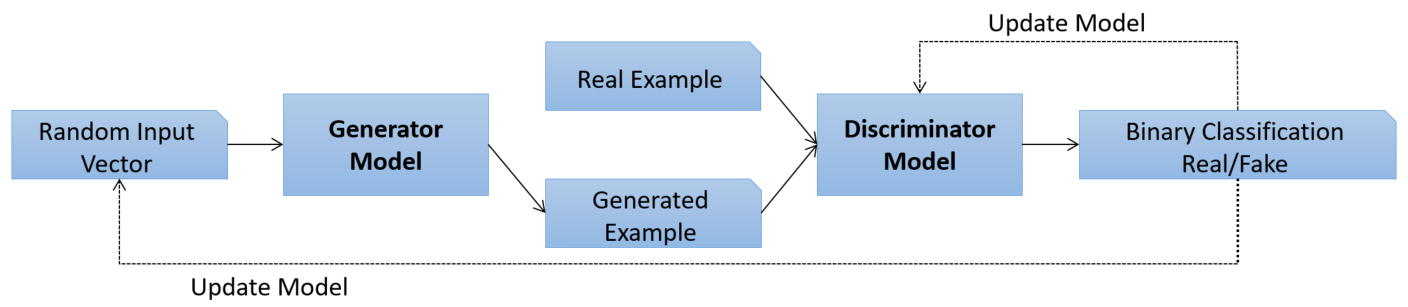
\includegraphics[width=.9\textwidth]{Chapters/figures/gan.PNG}
    \caption{Basic GAN model architecture}
\end{figure}
%

In this thesis the results of our score-based generative semantic image synthesis model are compared with the results of state-of-the-art GANs. All GAN models used for comparison are briefly explained below:

\subsection{Cascaded Refinement Networks}
\subsection{pix2pixHD} 
\subsection{SPADE} 


\section{Ganze viele Sections}
\section{Improvements and Adaptations}
\subsection{Solving reverse SDEs - Gotta go fast} %1-1.5
\subsection{Mixed precision learning} %0.5-1
\subsection{Training on arbitrary image sizes} %0.5-1

\chapter{Implementation and Experiments}
\section{Controllable Generation} %0.5-1
\section{Class-Conditional Sampling} %0.5-1
\section{Semantic Synthesis Sampling} %1-2
\section{A competitive experiment on the Cityscapes dataset} %5-7
\section{Generating high resolution landscapes} %5-7

\chapter{Conclusions and outlook} %2-3
%min 32 max 47
\appendix 
\bibliography{bibliography}
\addcontentsline{toc}{chapter}{Bibliography}

\end{document}
